\chapter{UJI COBA}

Pada bab ini dijelaskan tentang uji coba dan evaluasi dari implementasi yang telah dilakukan pada Tugas Akhir ini.

\section{\quad Lingkungan Uji Coba}
\quad Perangkat keras yang digunakan adalah \textit{Processor} AMD A8-6410 4 Cores 2.0 Ghz up to 2.4 GHz dengan \textit{random access memory}(RAM) sebesar 8 Gb. Dengan sistem operasi Windows 8.1 64 bit. Bahasa yang digunakan adalah bahasa C++ dengan bantuan \textit{integrated development environment}(IDE) Orwell Bloodshed Dev-C++ 5.11 serta compiler g++ (TDM-GCC 4.9.2 64-bit).
\section{\quad Skenario Uji Coba}
\quad Pada subbab ini akan dijelaskan skenario uji coba yang dilakukan.
	\subsection{\quad Uji Coba Kebenaran}
		
		\subsubsection{\quad Uji Coba Kebenaran Penyelesaian Permasalahan \textit{LIS and TREE by value}}
		\quad Uji coba kebenaran dilakukan dengan mengirimkan kode ke situs penilaian daring SPOJ sebanyak 20 kali pengiriman, ditunjukkan pada Gambar \ref{figure:accST}. Dari hasil uji yang dilakukan dapat dilihat bahwa kode sumber yang dikirimkan mendapat keluaran \textit{Accepted} dengan waktu tercepat program adalah 1.81 detik dan memori yang dibutuhkan konstan pada besaran 41 MB.
		\begin{figure}[H]
			\centerline{ 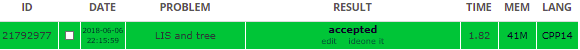
\includegraphics[scale=0.39]{assets/images/valueacc.png}}
			\caption{Hasil uji coba permasalahan \textit{LIS and TREE} pada situs penilaian daring SPOJ}
			\label{figure:accST}
		\end{figure}
		\subsubsection{\quad Uji Coba Kebenaran Penyelesaian Permasalahan \textit{LIS and TREE by reference}}
		\quad Uji coba kebenaran dilakukan dengan mengirimkan kode ke situs penilaian daring SPOJ sebanyak 20 kali pengiriman, ditunjukkan pada Gambar \ref{figure:accP}. Dari hasil uji yang dilakukan dapat dilihat bahwa kode sumber yang dikirimkan mendapat keluaran \textit{Accepted} dengan waktu tercepat program adalah 0.66 detik dan memori yang dibutuhkan rata-rata sebesar 41 MB.
		\begin{figure}[H]
			\centerline{ 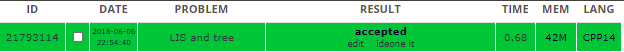
\includegraphics[scale=0.39]{assets/images/pointeracc.png}}
			\caption{Hasil uji coba permasalahan \textit{LIS and TREE} pada situs penilaian daring SPOJ}
			\label{figure:accP}
		\end{figure}
	\subsection{\quad Uji Coba Kinerja}
		
		\subsubsection{\quad Uji Coba Kinerja Pengaruh Jumlah Node Permasalahan \textit{LIS and TREE}}
		\quad Pada uji coba yang ditunjukkan Gambar \ref{figure:grafnode} terlihat performa program dengan input jumlah kasus uji satu, dan jumlah \textit{node} yang bertambah hingga 100000.
		\begin{figure}[H]
			\centerline{ 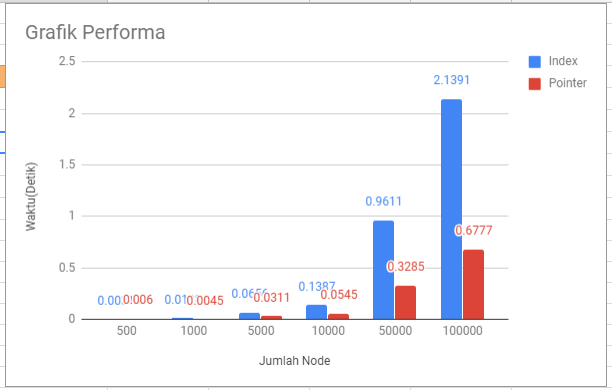
\includegraphics[scale=0.65]{assets/images/GrafikPerformaNode.PNG}}
			\caption{Hasil uji coba program menggunakan data dari generator}
			\label{figure:grafnode}
		\end{figure}
		\quad Pada gambar grafik berwarna merah menunjukkan performa dari implementasi menggunakan pointer dan warna biru menunjukkan performa dari implementasi menggunakan index. Terlihat perbedaan yang cukup besar ketika masukan mencapai 100000 \textit{node}, hal ini dikarenakan banyaknya bagian \textit{segment tree} yang kosong yang harus dicek pada saat menggunakan implementasi index.
		\subsubsection{\quad Uji Coba Kinerja Pengaruh Jumlah Kasus Uji Permasalahan \textit{LIS and TREE by reference}}
		\quad Pada uji coba yang ditunjukkan Gambar \ref{figure:graftestcase} terlihat performa program dengan input jumlah kasus uji yang bertambah hingga 1000, dan jumlah \textit{node} yang konstan yaitu 100000.
		\begin{figure}[H]
			\centerline{ 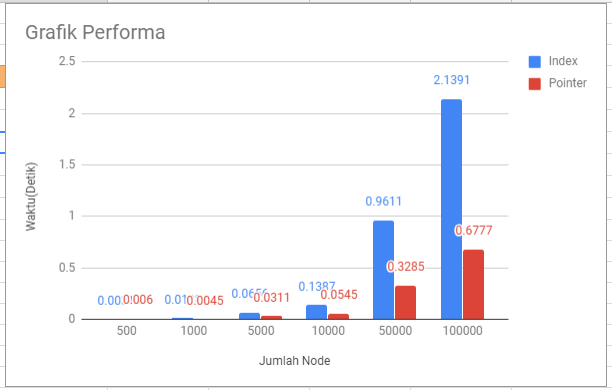
\includegraphics[scale=0.65]{assets/images/GrafikPerformaNode.PNG}}
			\caption{Hasil uji coba program menggunakan data dari generator}
			\label{figure:graftestcase}
		\end{figure}
		\quad Pada gambar grafik berwarna merah menunjukkan performa dari implementasi menggunakan pointer dan warna biru menunjukkan performa dari implementasi menggunakan index. Waktu disini bertambah seiring dengan banyaknya kasus uji secara konstan.